\section{Context-Free Grammar (\texttt{CFG})}
\label{cfg_chapter}

Recall that previous topics discussed regular models of computation; these are the finite-state machines (\texttt{FSA}; Mealy, Moore, \texttt{NFA}, \texttt{DDA}, among others) that define a \blue{regular language}.

A \textbf{Context-Free Language} is another type of model of computation that can be generated by a \texttt{CFG}.

\paragraph{Formal Definition of a \texttt{CFG}.}  A \texttt{CFG} $G$ is a formal grammar that generates a string in its language $L(G)$ using a list of \blue{terminal} and \blue{non-terminal symbols}, and \blue{production rules}. Formally, it is defined as:

    \[
    G=\left(V,\Sigma, R,S\right)
    \]
    Where,
    \begin{itemize}
        \item $V$ is a finite set of non-terminal symbols, each $v\in V$ represents a \blue{phrase or clause in the sentence}.
        \item $\Sigma$ is a finite set of terminal symbols, that are the \blue{possible symbols or string}  of the generated sentence. The alphabet of the grammar $G$ is the set of terminal symbols. It must be the case that $\Sigma \cap V=\emptyset$.
        \item $R$ is a relation $V\times (V\cup\Sigma)^*$, which are the productions of the grammar. These are the \blue{rules for producing a sentence}.
        \item $S$ is the start string, used to represent the whole sentence. It must be the case that $S\in V$.
    \end{itemize}

\begin{defn}
    A \textbf{non-terminal symbol} (or \blue{variable}) is a symbol that can be \blue{expanded} using a production rule.
\end{defn}

\begin{defn}
    A \textbf{terminal symbol} is a symbol that \blue{}{cannot be expanded further}.
\end{defn}

\begin{defn}
    The \textbf{sentential form} is a string of \blue{terminals}, \blue{non-terminals}, or both. 
\end{defn}

\begin{defn}
    Given two sentential forms $w$ and $w^\prime$, if $w$ can be transformed to $w^\prime$ using one production rule. Therefore, $w^\prime$ is \textbf{immediately derivable} from $w$, or $w\Rightarrow w^\prime$.
\end{defn}

\begin{defn}
    A sentential form that is composed of all \blue{terminal symbols} is a \textbf{sentence} $\Sigma \overset{*}{\Rightarrow} w\in L(G)$.
\end{defn}

\paragraph{Formal Definition of a Context-Free Language.} The language of $G=\left(V,\Sigma,R,S\right)$, then $L(G)=\left\{s\in\Sigma|S\overset{*}{\Rightarrow}w\right\}$. It is the set of all terminal-symbol strings derivable from the start symbol.  A language $L$ is a Context-Free Language (CFL) if it meets the criteria: 

\[
\exists M, L(M)=L \Longleftrightarrow L\text{ is a CFL}
\]

\begin{ex}
    The grammar $G$ is a grammar that can produce the following strings:
\end{ex}
\begin{itemize}
    \item A man.
    \item A woman.
    \item The kid.
    \item The child.
\end{itemize}

We first determine the general structure of $G$. We see that a sentence contains two words. Denote the first word in the sentence as \textsc{Article} and the second word be \textsc{Noun}. It follows that we have the sentence structure

\[
    S\to \textsc{Article} \cdot p \cdot \textsc{ Noun}
\]

As a side note, we use $p$ as the blank symbol, or the non-terminal for the whitespace character. With the sentence structure and non-terminal symbols defined, we can populate the set of terminal symbols given the sample sentences:

\begin{center}
    \begin{tabular}{cl}
         \textsc{Article} & \{"A", "The"\}  \\
         \textsc{Noun}    & \{"man, "woman", "kid", "child"\}
    \end{tabular}
\end{center}

Then, we can now create the production rules for $G$:

\begin{center}
    \begin{tabular}{rl}
         $S \to$                & \textsc{Article} p \textsc{Noun} \\
         \textsc{Article} $\to$ & \{"A", "The"\} \\
         \textsc{Noun}    $\to$ & \{"man, "woman", "kid", "child"\}\\
         $p \to$                & " " 
    \end{tabular}
\end{center}

\subsection{Parse Trees and Ambiguity}

A \blue{specific derivation} of a string from a grammar $G$ can be represented as a parse tree.

\begin{defn}
    A parse tree is a tree-structure where the root element is the String structure that branches out for every \blue{non-terminal symbol} in the derived string. See \ref{parse_tree_sample} for an example.
\end{defn}

\begin{figure}
    \centering
    \label{parse_tree_sample}
    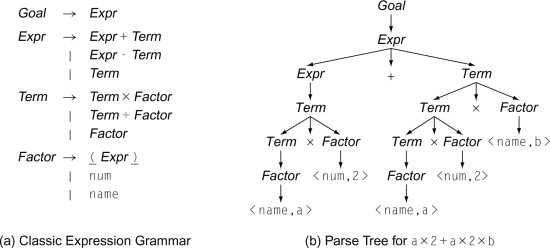
\includegraphics[width=0.75\linewidth]{images/parse_tree_sample.jpg}
\end{figure}

\begin{defn}
    Suppose we have a grammar $G$ has the sentence structure $S=R_1 R_2$ which has two \blue{productions}: $R_1 \to 0R_11 | 01$ and $R_2 \to 1R_2\texttt{x} | 1\texttt{x}$.

    \begin{enumerate}
        \item The \textbf{leftmost derivation} is the derivation which primarily expands the leftmost non-terminal symbols for each production.
        \item The \textbf{rightmost derivation} is the derivation which primarily expands the rightmost non-terminal symbols for each production.
    \end{enumerate}
\end{defn}

\begin{defn}
    A grammar $G$ is ambiguous if and only if $\exists w\in L(G)$ has multiple \blue{leftmost} derivations.
\end{defn}